\documentclass[../../main.tex]{subfiles}
\begin{document}

\subsection*{10.1}
Una sbarretta conduttrice di lunghezza b si muove con velocità v costante e ortogonale ad un filo rettilineo indefinito per corso dalla corrente i.\\
Calcolare la tensione ai cai della sbarretta in funzione della distanza r dal filo.\\
Ripetere il calcolo quando la sbarretta si muove con velocità costante parallela al filo e l'estremo più vicino al filo dista da r.\\
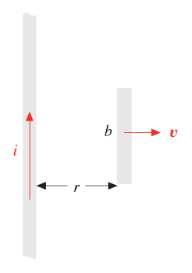
\includegraphics[scale=0.3]{e_10_1_0.png}
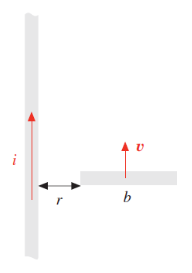
\includegraphics[scale=0.3]{e_10_1_1.png}
\subsubsection*{Formule utilizzate}
\subsubsection*{Soluzione punto a}
$\vec{E_i} = \frac{\vec{F}}{q} = \vec{v}\wedge\vec{B}$\\
Per la legge di Biot-Savart $\vec{B} = \frac{\mu_0i\vec{u_\phi}}{2\pi r}$\\
Integradno su tutta la barra lunga b, otteniamo la forza elettromotrice $\varepsilon_1 = \int_o^b\vec{E_i}d\vec{s} = \int_0^b\vec{v}\wedge\vec{B} ds = \frac{\mu_0ivb}{2\pi r}$\\
Analogamente: $\varepsilon_2 = \int_r^{r+b} \vec{E_i} d\vec{s} = \int_r^{r+b}\vec{v}\wedge\vec{B} ds= -\frac{\mu_0 iv}{2\pi}\int_r^{r+b}\frac{dr}{r} = -\frac{\mu_0 iv}{2\pi}ln\left(1+\frac{b}{r}\right)$\\
Il segno indica che ha potenziale maggiore l'estremo più vicino al fino.\\
\subsubsection*{Soluzione punto b}
Si scriva lo stesso risultato anche ragionando con il flusso tagliato, ovvero tenuto conto che il flusso $\Phi$ è il prodotto del campo magnetico B per l'area $\Sigma$ che viene "tagliata" dal flusso.\\
$\Phi = \int_\Sigma\vec{B}\vec{u_n}d\Sigma$\\
$B = \frac{\mu_0i}{2\pi r}$\\
$d\Sigma = bdx$
\tab $d\Phi = \frac{\mu_0i}{2\pi r}bdx$\\
$\Phi = \frac{\mu_0 ib}{2\pi r}\int_0^xdx = \frac{\mu_0 ibx}{2\pi r}$\\
$\varepsilon_1 = \frac{d\Phi}{dt} = \frac{\mu_0 ib}{2\pi r}v$\\\\
Utilizzando il flusso tagliato con $d\Sigma = ydr$:\\
$d\Phi = \frac{\mu_0iy}{2\pi r}ydr$\\
$\Phi = \frac{\mu_0 iy}{2\pi}\int_r^{r+b}\frac{dr}{r} = \frac{\mu_0 iy}{2\pi}ln\left(1+\frac{b}{r}\right)$\\
$\varepsilon_2 = \frac{d\Phi}{dt} = \frac{\mu_0i}{2\pi}v\ ln\left(1+\frac{b}{r}\right)$
\newpage
\end{document}